\documentclass{beamer}
\usepackage[utf8]{inputenc}
\usepackage[german]{babel}
\usepackage[T1]{fontenc}
\usepackage{amsmath}
\usepackage{amsfonts}
\usepackage{amssymb}
\usepackage{booktabs}
\usepackage{graphicx}
\usepackage{enumitem}
\usepackage{csquotes}
\usepackage{lmodern}
\usepackage{pifont}
\usepackage{hyperref}


%Navigationsleiste verschwinden lassen
\beamertemplatenavigationsymbolsempty

% \logo{\includegraphics[height= 0.5 cm]{Franz}}
\title[Soziale Ungleichheit in der Lebenserwartung]{Soziale Ungleichheit der Lebenserwartung in Deutschland}
%\institute{wissenschaftliches Arbeiten, TU Dortmund}
\author{Caroline Baer, Louisa Poggel}
\date{07. Dezember 2021}

\usetheme{CambridgeUS}
\usecolortheme{dolphin} %oder beaver oder crane (update 27.11, 13:29)
\useinnertheme{rounded}

\begin{document}

\begin{frame}
 \maketitle
\end{frame}

\begin{frame}
 \frametitle{Inhaltsverzeichnis}
  \tableofcontents  %[pausesections]
\end{frame}

\section{Motivation}
\begin{frame}{Veränderung der Lebenserwartung}
	\begin{block}{}
		\begin{itemize}
		\item[$\blacktriangleright$] 1880: nur ein Drittel der Bevölkerung erreicht das 60. Lebensjahr
		\item[$\blacktriangleright$] 1975: sind es bereits 75\%
%zu volle Folie	\item[$\blacktriangleright$] Ende 20.Jhd: nahe 90 \%
		\item[$\blacktriangleright$] weiterer Anstieg erwartet
		\end{itemize}
	\end{block}
	\pause
	\begin{block}{}
		\begin{itemize}
			\item[$\blacktriangleright$] 2005: 19\% der Gesamtbevölkerung älter als 65
			\item[$\blacktriangleright$] Vorausrechnung des Statistischen Bundesamtes\\ für 2050: 30\% älter als 65
		\end{itemize}
	\end{block}
	\pause
	\begin{block}{Gründe:}
		\begin{itemize}
			\item[$\blacktriangleright$] Eindämmung der Infektionskrankheiten und Kindersterblichkeit
			\item[$\blacktriangleright$] Verringerung chronischer Krankheit im hohen Alter
			\item[$\blacktriangleright$] bessere Lebensbedingungen
		\end{itemize}
	\end{block}
\end{frame}

\begin{frame}
 \frametitle{Unterschiede in der Lebenserwartung}
\textbf{Differenz mittlere Lebenserwartung bei Geburt:}

niedrigste Einkommensgruppe \hfill höchste Einkommensgruppe

\hspace{1.5cm}
\includegraphics[height=2cm]{Personen}\hspace{2cm} 
$\Longleftrightarrow$ \hspace{2cm}
\includegraphics[height=2cm]{Personen}\\
\vspace{0.5cm}
\hspace{4.3cm} \textbf{Frauen: 4.4 Jahre}\\
\hspace{4.3cm} \textbf{Männer: 8.6 Jahre}
     
    
\end{frame}

\section{Hypothese}
\begin{frame}
 \frametitle{Hypothese: Lebenserwartung in Deutschland vom Einkommen stark beeinflusst}
 \textbf{Ungleichheit der Lebensbedingungen:}
 \vspace{0.5cm}
 \begin{itemize}
   \item [$\blacktriangleright$] Verteilung des Einkommens
   \item [$\blacktriangleright$] Bildungschancen
   \item [$\blacktriangleright$] Risiko chronischer Erkrankungen
   \item [$\blacktriangleright$] individuelles Gesundheitsverhalten
 \end{itemize}
 \vspace{0.5cm}
 $\rightarrow$ Verkürzte Lebenszeit sozial benachteiligter Bevölkerungsgruppen
 
\end{frame}


\section{Studie und Datenbasis}
\begin{frame}
\frametitle{Wichtige Datenquellen und Studien}
  \begin{block}{Sozio-oekonomische Panel (SOEP)}
   \begin{itemize}
     \item [$\blacktriangleright$] durch Deutsches Institut für   Wirtschaftsforschung (DIW)
     \item [$\blacktriangleright$] Panelstudie von 1992-2016
     \item [$\blacktriangleright$] Daten von  83.287 Personen (bezüglich obigen Zeitraumes)
 %   \item[$\blacktriangleright$] jährliche Haushaltsbefragung
     \item[$\blacktriangleright$] insgesamt 4.193 (dh. 5\%) Studienteilnehmer im beobachteten Zeitraum verstorben
   \end{itemize}
  \end{block}
  \begin{block}{Daten des Statistischem Bundesamt}
   \begin{itemize}
     \item [$\blacktriangleright$] Amtliche Periodensterbetafeln
     \item [$\blacktriangleright$] Statistik der natürlichen Bevölkerungsbewegung
   \end{itemize}
  \end{block}
\end{frame}


\section{Verwendete Methoden}
\begin{frame}{Netto-Äquivalenzeinkommen}
	\begin{itemize}
		\item[$\blacktriangleright$] Einkommen nach Berücksichtigung von Größe/Zusammensetzung des Haushaltes, sowie unterschiedlichen Einkommensbedarfes
\vspace{0.3cm}		
		\begin{itemize}
		\item[$\rightarrow$]	Addition des Einkommen des gesamten Haushalts \& Gewichtung nach neuer OECD-Skala
		\item[$\rightarrow$] Gewichtung nach Anzahl und Alter der Personen gerichtet
\vspace{0.2cm}
		\item[$\Rightarrow$] Netto-Äquivalenzeinkommen$=\frac{\text{Summe der Nettoinkommen (in €)}}{\text{Summe der Personengewichte}}$
		\end{itemize}
\vspace{0.3cm}
		\item[$\blacktriangleright$] 2005: mittlere Netto-Äquivalenzeinkommen $=$1.398€
	\end{itemize}
\end{frame}

\begin{frame}{Einkommensgruppen}
	\begin{block}{Einteilung in 5 Gruppen bzgl. des gesellschaftlichen Medians:}
		\begin{itemize}
			\item[$\blacktriangleright$] unter 60\%
			\item[$\blacktriangleright$] 60 bis unter 80\%
			\item[$\blacktriangleright$] 80 bis unter 100\%
			\item[$\blacktriangleright$] 100 bis unter 150\%
			\item[$\blacktriangleright$] über 150\%
		\end{itemize}
	\end{block}
	\begin{block}{Schwellenwerte von 2005:}
		\begin{itemize}
			\item[$\blacktriangleright$] 60\%: 839€ \\ $\rightarrow$ nach sozialpolitischer Definition von Armut betroffen oder gefährdet
			\item[$\blacktriangleright$] 150\%: 2.097€
		\end{itemize}
	\end{block}
\end{frame}



\section{Ergebnisse}
\begin{frame}
\textbf{Überlebensraten nach Geschlecht und Einkommen}
	\includegraphics[scale=0.18]{Abb.2_Überlebensraten nach Geschlecht und Einkommen_korrigiert}
\end{frame}

\begin{frame}
	\includegraphics[scale=0.17]{Abb.3_Mortalitätsrisiko vor einem Alter von 65 Jahren}
\end{frame}

\begin{frame}
	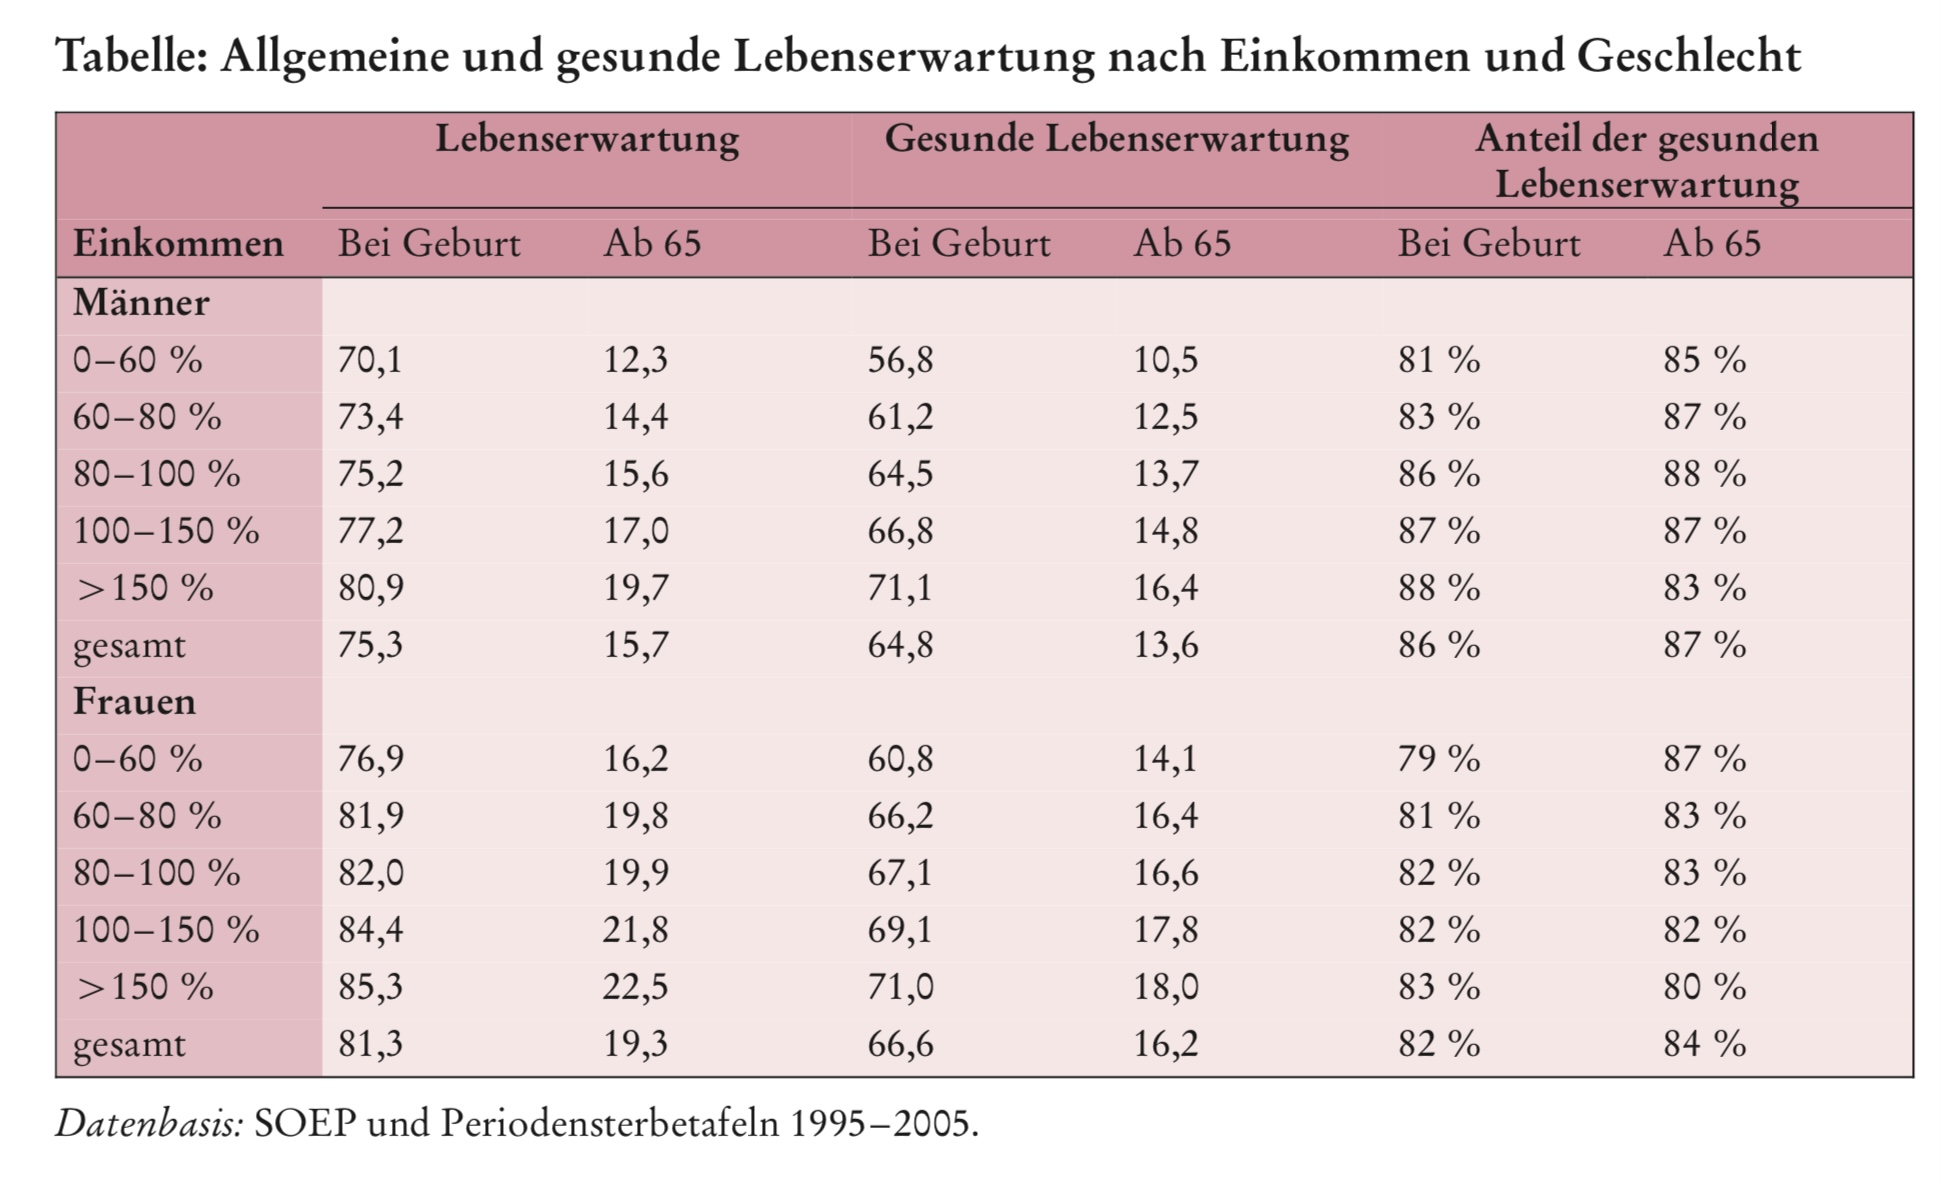
\includegraphics[scale=0.18]{Tabelle_allgemeine und gesunde Lebenserwartung}
\end{frame}

%--------------richtiger Ort?--------soll diese Folie drin bleiben?----------
\begin{frame}
\frametitle{Herausforderungen bei Datenerhebung und statistischer Analyse}
	\begin{itemize}
		\item [$\blacktriangleright$] keine amtliche Informationsquelle die 	Sterberegister mit sozialer Lage verknüpft
		\item [$\blacktriangleright$] Austretende Studienteilnehmer (mit schlechter Gesundheit)
			\begin{itemize}
				\item $\rightarrow$ Unterschätzung Mortalität
				\item $\rightarrow$ Überschätzung Lebenserwartung
			\end{itemize}
		\item [$\blacktriangleright$]Theorie: Erhöhung der Lebenszeit in höchsten/mittleren Einkommensklassen stärker als in niedrigster Einkommensklasse
		\begin{itemize}
			\item $\rightarrow$ keine statistische Absicherung aufgrund zu niedriger\\
			\hspace{0.4cm} Fallzahlen (große Unsicherheit der Schätzer)
		\end{itemize}
	\end{itemize}
\end{frame}
%----------------------------------------
 
 
\section{Fazit}
\begin{frame}{Fazit: Lebenserwartung}
	\begin{block}{Veränderung der Lebenserwartung im Beobachtungszeitraum:}
		\begin{itemize}
			\item[$\blacktriangleright$] Frauen: 78,9 $\rightarrow$ 82,2 Jahre\\
			\begin{itemize}
			\item[$\bullet$] 1,4 Jahre Zugewinn (niedrigste Einkommensgruppe)
			\item[$\bullet$] 3,9 Jahre Zugewinn (höchste Einkommensgruppe)
			\end{itemize}								
			\item[$\blacktriangleright$] Männer: 72,3 $\rightarrow$ 77,4 Jahre
			\begin{itemize}
				\item[$\bullet$] 4,2 Jahre Zugewinn (niedrigste Einkommensgruppe)
				\item[$\bullet$] 6,9 Jahre Zugewinn (höchste Einkommensgruppe)
			\end{itemize}
		\end{itemize}
	\end{block}
	\pause
	\begin{block}{Differenz zwischen niedrigster und höchster Einkommensgruppe}
		\begin{itemize}
			\item[$\blacktriangleright$] bzgl. mittlerer Lebenserwartung bei Geburt:\\ Frauen: 4,4 Jahre, Männer: 8,6 Jahre
			\item[$\blacktriangleright$] bzgl. fernerer Lebenserwartung ab einem Alter von 65 Jahren:\\ Frauen: 3,7 Jahre, Männer: 6,6 Jahre
		\end{itemize}
	\end{block}
\end{frame}

\begin{frame}{Fazit: Mortatlitätsrisiko}
	\begin{block}{}
		\begin{itemize}
			\item[$\blacktriangleright$] 13,2\% der Frauen, 27,2\% der Männer aus der niedrigsten Einkommensgruppe sterben vor Vollendung des 65. Lebensjahres
			\item[$\blacktriangleright$] 8,2\% der Frauen, 13,6\% der Männer aus der höchsten Einkommensgruppe sterben vor Vollendung des 65. Lebensjahres
		\end{itemize}
	\end{block}
	\pause
	\begin{block}{Mortalitätsrisiko in der niedrigsten Einkommensgruppe}
		\begin{itemize}
			\item[$\blacktriangleright$] bis zum Alter von 50 Jahren:
			\begin{itemize}
				\item[$\bullet$] Frauen: 2,2-fach höher, Männer: 2,4-fach höher
			\end{itemize}
			\item[$\blacktriangleright$] ab einem Alter von 51 Jahren:
			\begin{itemize}
				\item[$\bullet$] Frauen: 1,5-fach, Männer: 1,9-fach höher 
			\end{itemize}
		\end{itemize}
	\end{block}
\end{frame}


\section{Quellen}
\begin{frame}
\frametitle{Quellen}
  \begin{itemize}
    \item \textbf{Symbolbild Personen:}
    https://icon-icons.com/de/symbol/Benutzer-Gruppe-Personen-   Kunden-Klienten/72448
  \end{itemize}

\end{frame}


\section{Diskussion}
\begin{frame}
	\begin{block}{Frage 1:}
		 Was glaubt ihr wie sich die Lebenserwartung in den nächsten Jahren entwickeln wird?
	\end{block}
	\pause  %zweite Frage erst nach Diskussion erster Frage einblenden
	\begin{block}{Frage 2:}
		 Habt ihr Vorschläge wie man die soziale Ungleichheit in der Lebenserwartung verringern oder gar aufheben könnte?
	\end{block}
\end{frame}



\end{document}